\documentclass{homework}
\usepackage[utf8]{inputenc}

\usepackage{graphicx}
\graphicspath{ {./images/} }

\usepackage[fleqn]{amsmath}
\usepackage{amssymb}

\title{GPGN470A HW 2: EM Radiation}
\author{Tyler Singleton}

\begin{document}
\maketitle

Question 1: \\ \\
Yes. While both the field grass and surrounding grass display a strong green reflection, there is an obvious visual difference in composition present in the second image. The surrounding grass and natural vegetation have a significant difference in spectral response in the near-infrared than the field grass. So the conclusions I draw from this is that field grass and surrounding grass have a different material composition. Knowing artificial turf is commonly utilized within sport centers, I could assume this to be such a case. However, other cases also exist. Such as it could be a  different grass species, but I do not believe this to be probable as the surrounding foliage displays a similar response to the surrounding natural grass. \\

%-----------------------------------------------%

Question 2: \\ \\
(a)
\begin{figure}[h]
    \centering
    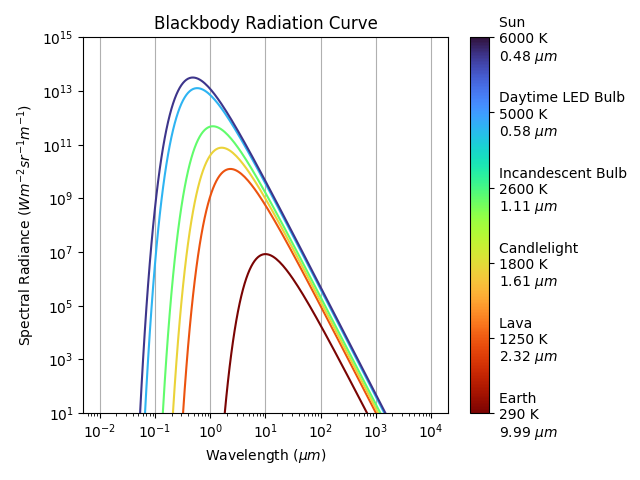
\includegraphics[width=0.75\textwidth]{Blackbody_Curve.png}
    \caption{This figure shows the blackbody radiation curve for Earth at $290 K$, Lava at $1250 K$, Candlelight at $1800 K$, Incandescent Bulb at $2600 K$, Daytime LED Bulb at $5000 K$, and the Sun at $6000 K$. Their respective wavelength at peak spectral radiance was calculated and illustrated on the color bar.}
    \label{fig:blackbody}
\end{figure}

(b)
To observe lava, I would stay mostly in the infrared/near-infrared band between $7 \mu m$ and $1 \mu m$. The reason for this, is that there is significant difference in spectral radiance between earth and lava. Although earth peaks around $10 \mu m$, there is roughly a 3 magnitude difference in spectral radiance between the two. Approaching the near-infrared band, the spectral radiance of earth quickly approaches 0. \\

For this, I would prefer to use a satellite based platform. Between $4 \mu m$ and $7 \mu m$, there is very little absorption from the atmosphere. Additionally, I could expect little Rayleigh scattering which is the predominate form of scattering in our atmosphere. Accessibility is another reason. Lava flow can be dangerous, so installing and monitoring ground based equipment is hazardous and unfeasible during periods of significant volcanic activity. Moreover, the limited viewing angles reduce the field of view that can be observed. Airborne is also not considered to be optimal. As with ground-based stations, periods of significant volcanic activity create hazardous flying conditions, although higher altitudes may circumvent this. Additionally, the temporal resolution for airborne would be too low as lava flows may change directions quickly. \\

(c)
Advances in technology have allowed us to use illumination that is more closely representative of the sun's radiance, and also much more efficient in that the spectral radiance peaks along the visual spectrum. Thus, less energy is wasted. \\

%-----------------------------------------------%

Question 3: \\ \\
(a) 
\begin{equation*}
    \begin{split}
        S_{sun} 
        & = \sigma T^4 \\
        & \approx (5.67*10^{-8}Wm^{-2}K^{-4})(5800K)^4 \\
        & \approx 6.42*10^{7}Wm^{-2}
    \end{split}
\end{equation*}
    
    
(b)
\begin{equation*}
    \begin{split}
        S 
        & = S_{sun}(\frac{r_{sun}}{D})^2 \\
        & = 6.42*10^7 Wm^{-2}(\frac{6.96*10^5 km}{1.50*10^8 km})^2 \\
        & = 1.38*10^3 Wm^{-2}
    \end{split}
\end{equation*}
    
(c)
\begin{equation*}
    \begin{split}
        P_{incident} 
        & = SA_{surface} = S4 \pi r^2_{earth} \\
        & = (1.38*10^3 Wm^{-2})(4 \pi)(6.378*10^6 m)^2 \\
        & = 7.05*10^{17} W 
    \end{split}
\end{equation*}
Since the earth is a sphere, only about 1/4 of the surface will absorb the solar radiance due to angular distributions (Rees 2.5). Therefore, 
\begin{equation*}
    P_{incident} = 1.76*10^{17} W
\end{equation*}

(d) 
\begin{equation*}
    P_{absorbed} = (1-\alpha) P_{incident} = (0.7)(1.76*10^{17} W) = 1.23*10^{17} W
\end{equation*}

(e)
\begin{equation*} P_{incident} = P_{absorbed} + P_{reflected} \end{equation*}
\begin{equation*} \therefore \end{equation*}
\begin{equation*}
    \begin{split}
        P_{absorbed} 
            & = P_{incident} - P_{reflected} = (\sigma T^4) (\frac{r_{sun}}{D})^2 (\pi r^2_{planet})(1-\alpha)
    \end{split}
\end{equation*}

(f)
\begin{equation*}
    \begin{split}
        T 
            & =\left[ (\frac{P_{absorbed}}{4\pi r^2_{earth}})(\frac{1}{\sigma})             
            \right]^\frac{1}{4} \\
            & =\left[ (\frac{1.23*10^{17}W}{4\pi*(6.378*10^{6}m)^2})(\frac{1}{5.67*10^{-8} Wm^{-2}K^{-4}}) \right]^\frac{1}{4} \\
            & = 255 K
    \end{split}
\end{equation*}

(g)
The global average temperature of earth is $288K$ which is similar, but slightly higher than the expected temperature of $255K$. This tells me that earth is relatively in equilibrium with its blackbody radiation. Additionally, the measured temperature being slightly higher makes sense. The earth is also radiating heat from its core, to the surface, then the atmosphere -- this could account for a small difference. However, the atmosphere acts as a great insulator preventing radiated surface heat from escaping and this mostly accounts for the difference and observed temperatures.\\

(h)
\begin{equation*}
    T_{Mercury} =\left[ \frac{(5800K)^4(6.96*10^8 m)^2 (1-0.10)}{4*(5.79*10^{10} m)^2}         \right]^\frac{1}{4} = 438 K 
\end{equation*}

\begin{equation*}
    T_{Venus} =\left[ \frac{(5800K)^4(6.96*10^8 m)^2 (1-0.75)}{4*(1.082*10^{11} m)^2}
    \right]^\frac{1}{4} = 233 K 
\end{equation*}

\begin{equation*}
    T_{Mars} =\left[ \frac{(5800K)^4(6.96*10^8 m)^2 (1-0.25)}{4*(2.279*10^{11} m)^2}         
    \right]^\frac{1}{4} = 211 K
\end{equation*}

For Mercury, the observed surface temperature and blackbody temperature are relatively close; in addition to having a low albedo, Mercury closely resembles a blackbody. For Venus, its observed temperature has greatly exceeded the blackbody temperature. This can be attributed to Venus' thick atmospheric composition. Although highly reflective, Venus' atmosphere is efficient in preventing escaping radiation. Finally, for Mars, both temperatures are nearly identical. This is characteristic of Mars' atmosphere inability to significantly absorb heat.


\end{document}
